\documentclass[notitlepage,aps,prd,nofootinbib]{revtex4-1}

\usepackage{subfig}
%\usepackage[colorinlistoftodos]{todonotes}
\usepackage{float}

%\usepackage[protrusion=true,expansion=true]{microtype}
\usepackage{amsmath}
\usepackage{amssymb}
\usepackage{bbm}
\usepackage{ulem}
%\usepackage{feynmp-auto}
%\usepackage{slashed}
%\usepackage[absolute,overlay]{textpos}
\usepackage[usenames, dvipsnames]{color}
\usepackage{graphicx}
\usepackage{listings}
\usepackage{epsfig}
\usepackage{hyperref}
%\usepackage{tikz}
\usepackage{enumerate}
%\usepackage{fixltx2e} % buggy
\usepackage[compatibility=false]{caption}
%\usepackage{subcaption} % doesn't work with subfigure
\usepackage{pdfpages}
%\usepackage{setspace}
\usepackage{verbatim}

% Turn off meaningless float warnings
\usepackage{silence}
\WarningFilter{revtex4-1}{Repair the float}

\DeclareRobustCommand{\orderof}{\ensuremath{\mathcal{O}}}

\definecolor{dukeblue}{RGB}{0,0,156}
\definecolor{dukedarkblue}{RGB}{0,26,87}
\definecolor{dukeblack}{RGB}{79,79,79}
\definecolor{dukegray}{RGB}{79,79,79}
\definecolor{dukesecbrown}{RGB}{217,200,158}
\definecolor{dukesecblue}{RGB}{127,169,174}

%\renewcommand*{\thefootnote}{\fnsymbol{footnote}}

%%%%%%%%%%%%%%%%%%%%%%%%%%%%%%%%%%%%%%%%%%%%%%%%%%%%%%%%%%%%%%%%%%%%%%%%%%%%%%%%%%%%%
\hypersetup{
    breaklinks,
    baseurl       = http://,
    pdfborder     = 0 0 0,
    pdfpagemode   = UseNone,% do not show thumbnails or bookmarks on opening
    pdfstartpage  = 1,
    bookmarksopen = true,
    bookmarksdepth= 2,% to show sections and subsections
% revtex needs author and title declared after \begin{document}, so have to hard code them...
%    pdfauthor     = {\@author},
%    pdftitle      = {\@title},
    pdfauthor     = {Matthew Epland},
    pdftitle      = {Phys 566 HW5},
    pdfsubject    = {},
    pdfkeywords   = {}}


% Code import settings
%%%%%%%%%%%%%%%%%%%%%%%%%%%%%%%%%%%%%%%%%%%%%%%%%%%%%%%%%%%%%%%%%%%%%%%%%%%%%%%%%%%%%
\definecolor{mygreen}{rgb}{0,0.6,0}
\definecolor{mygray}{rgb}{0.5,0.5,0.5}
\definecolor{mymauve}{rgb}{0.58,0,0.82}

%\lstset{ %
\lstdefinestyle{python}{ %
  backgroundcolor=\color{white},   % choose the background color; you must add \usepackage{color} or \usepackage{xcolor}
  basicstyle=\scriptsize,          % the size of the fonts that are used for the code
  breakatwhitespace=false,         % sets if automatic breaks should only happen at whitespace
  breaklines=true,                 % sets automatic line breaking
  captionpos=b,                    % sets the caption-position to bottom
  commentstyle=\color{mygreen},    % comment style
  deletekeywords={...},            % if you want to delete keywords from the given language
  escapeinside={\%*}{*)},          % if you want to add LaTeX within your code
  extendedchars=true,              % lets you use non-ASCII characters; for 8-bits encodings only, does not work with UTF-8
  frame=single,	                   % adds a frame around the code
  keepspaces=true,                 % keeps spaces in text, useful for keeping indentation of code (possibly needs columns=flexible)
  keywordstyle=\color{blue},       % keyword style
  language=Python,                 % the language of the code
  otherkeywords={*,...},           % if you want to add more keywords to the set
  numbers=left,                    % where to put the line-numbers; possible values are (none, left, right)
  numbersep=5pt,                   % how far the line-numbers are from the code
  numberstyle=\tiny\color{mygray}, % the style that is used for the line-numbers
  rulecolor=\color{black},         % if not set, the frame-color may be changed on line-breaks within not-black text (e.g. comments (green here))
  showspaces=false,                % show spaces everywhere adding particular underscores; it overrides 'showstringspaces'
  showstringspaces=false,          % underline spaces within strings only
  showtabs=false,                  % show tabs within strings adding particular underscores
  stepnumber=5,                    % the step between two line-numbers. If it's 1, each line will be numbered
  stringstyle=\color{mymauve},     % string literal style
  tabsize=2,	                   % sets default tabsize to 2 spaces
%  title=\lstname                   % show the filename of files included with \lstinputlisting; also try caption instead of title
  title={\protect\filename@parse{\lstname}\protect\filename@base.\filename@ext},
  firstnumber=0,
%  linewidth=0.95\textwidth
  xleftmargin=0.01\textwidth,
  xrightmargin=0.01\textwidth
}

\lstdefinestyle{output}{ %
  backgroundcolor=\color{white},   % choose the background color; you must add \usepackage{color} or \usepackage{xcolor}
  basicstyle=\scriptsize,          % the size of the fonts that are used for the code
  breakatwhitespace=false,         % sets if automatic breaks should only happen at whitespace
  breaklines=true,                 % sets automatic line breaking
  captionpos=b,                    % sets the caption-position to bottom
  escapeinside={\%*}{*)},          % if you want to add LaTeX within your code
  frame=single,	                   % adds a frame around the code
  keepspaces=true,                 % keeps spaces in text, useful for keeping indentation of code (possibly needs columns=flexible)
  numbers=left,                    % where to put the line-numbers; possible values are (none, left, right)
  numbersep=5pt,                   % how far the line-numbers are from the code
  numberstyle=\tiny\color{mygray}, % the style that is used for the line-numbers
  rulecolor=\color{black},         % if not set, the frame-color may be changed on line-breaks within not-black text (e.g. comments (green here))
  stepnumber=5,                    % the step between two line-numbers. If it's 1, each line will be numbered
  tabsize=2,	                   % sets default tabsize to 2 spaces
%  title=\lstname                   % show the filename of files included with \lstinputlisting; also try caption instead of title
  title={\protect\filename@parse{\lstname}\protect\filename@base.\filename@ext},
  firstnumber=0,
%  linewidth=0.95\textwidth
  xleftmargin=0.01\textwidth,
  xrightmargin=0.01\textwidth
}

\newcommand{\degree}{\ensuremath{^{\circ}}}

% Select between raw and saved plots here
%\graphicspath{{../code/output/}}
\graphicspath{{../code/output/plots_for_paper/}}

%%%%%%%%%%%%%%%%%%%%%%%%%%%%%%%%%%%%%%%%%%%%%%%%%%%%%%%%%%%%%%%%%%%%%%%%%%%%%%%%%%%%%
\begin{document}

\title{PHYS 566 HW5}
\author{Matthew Epland}
\affiliation{Department of Physics, Duke University, Durham, NC 27707, USA}

\date{\today}

\begin{abstract}
% This assignment is so short the introduction is basically as good as an abstract...
\end{abstract}\maketitle

\section{Introduction}
\label{sec:intro}
Generating pseudorandom numbers is a very important component of computational physics, as having a supply of random numbers is essential to run Monte Carlo and random walk simulations. In this assignment the uniform random number generator in Python's \texttt{random} library\footnote{The library is primarily based on the Mersenne Twister algorithm coded in C, which produces 53-bit precision floats with a period of $2^{19937}-1$. See \url{https://docs.python.org/2/library/random.html} for more details.} was tested to verify that it produced a sufficiently uniform distribution. The uniform random numbers generated by \texttt{random} were also used to produce a pseudorandom Gaussian distribution with standard deviation $\sigma = 1$ via the Box--Muller transform. For both cases, the pseudorandom distributions matched the desired distributions extremely well.

\section{Theory}
\label{sec:theory}
\subsection{Box--Muller Transform}
\label{subsec:box_muller}
The Box--Muller transform takes two independent, uniformly distributed random numbers, $U_{1}$ and $U_{2}$, and transforms them into two independent, Gaussian distributed random numbers, $Z_{1}$ and $Z_{2}$ (\ref{eq:Zs}). As written (\ref{eq:Zs}) produces a Gaussian distribution with standard deviation $\sigma = 1$. It is beyond the scope of this assignment to detail how the Box--Muller transform works mathematically, but as will be seen in section~\ref{subsec:gaussian_results} below the transform works as described.

\begin{equation} \label{eq:Zs}
\begin{aligned}
Z_{1} &= \sqrt{-2\ln U_{1}} \cos\left(2\pi U_{2}\right) \\
Z_{2} &= \sqrt{-2\ln U_{1}} \sin\left(2\pi U_{2}\right)
\end{aligned}
\end{equation}

\section{Results}
\label{sec:results}
Both the uniform pseudorandom distributions, section~\ref{subsec:uniform_results}, and the Gaussian pseudorandom distributions, section~\ref{subsec:gaussian_results}, produced by \texttt{random} and the Box--Muller transform matched the exact distributions very well. In both cases fits were performed on the data, a linear fit for the uniform distribution and a Gaussian fit for the Gaussian distribution, to support this claim. As can be seen in the many following plots, the fits matched the data very well -- especially for runs with large numbers of trials, $N$, and appropriately sized bins, $\approx1\%$ range per bin.

\clearpage
\subsection{Uniform}
\label{subsec:uniform_results}

\begin{figure}[!htbc]
  \centering
  \includegraphics[width=.72\textwidth]{part_a/uniform_N_1000_bins_10.pdf}
	{\par\nobreak\rule[9pt]{35em}{0.5pt}\vspace{-5mm}}
	\caption{Uniform random number distribution with $N = 1000$ and $10$ bins.}
	\label{fig:uniform_N_1000_bins_10}
\end{figure}

\begin{figure}[!htbc]
  \centering
  \includegraphics[width=.72\textwidth]{part_a/uniform_N_1000_bins_20.pdf}
	{\par\nobreak\rule[9pt]{35em}{0.5pt}\vspace{-5mm}}
	\caption{Uniform random number distribution with $N = 1000$ and $20$ bins.}
	\label{fig:uniform_N_1000_bins_20}
\end{figure}

\begin{figure}[!htbc]
  \centering
  \includegraphics[width=.72\textwidth]{part_a/uniform_N_1000_bins_50.pdf}
	{\par\nobreak\rule[9pt]{35em}{0.5pt}\vspace{-5mm}}
	\caption{Uniform random number distribution with $N = 1000$ and $50$ bins.}
	\label{fig:uniform_N_1000_bins_50}
\end{figure}

\begin{figure}[!htbc]
  \centering
  \includegraphics[width=.72\textwidth]{part_a/uniform_N_1000_bins_100.pdf}
	{\par\nobreak\rule[9pt]{35em}{0.5pt}\vspace{-5mm}}
	\caption{Uniform random number distribution with $N = 1000$ and $100$ bins.}
	\label{fig:uniform_N_1000_bins_100}
\end{figure}

\clearpage

\begin{figure}[!htbc]
  \centering
  \includegraphics[width=.72\textwidth]{part_a/uniform_N_1E6_bins_10.pdf}
	{\par\nobreak\rule[9pt]{35em}{0.5pt}\vspace{-5mm}}
	\caption{Uniform random number distribution with $N = 10^6$ and $10$ bins.}
	\label{fig:uniform_N_1E6_bins_10}
\end{figure}

\begin{figure}[!htbc]
  \centering
  \includegraphics[width=.72\textwidth]{part_a/uniform_N_1E6_bins_20.pdf}
	{\par\nobreak\rule[9pt]{35em}{0.5pt}\vspace{-5mm}}
	\caption{Uniform random number distribution with $N = 10^6$ and $20$ bins.}
	\label{fig:uniform_N_1E6_bins_20}
\end{figure}

\begin{figure}[!htbc]
  \centering
  \includegraphics[width=.72\textwidth]{part_a/uniform_N_1E6_bins_50.pdf}
	{\par\nobreak\rule[9pt]{35em}{0.5pt}\vspace{-5mm}}
	\caption{Uniform random number distribution with $N = 10^6$ and $50$ bins.}
	\label{fig:uniform_N_1E6_bins_50}
\end{figure}

\begin{figure}[!htbc]
  \centering
  \includegraphics[width=.72\textwidth]{part_a/uniform_N_1E6_bins_100.pdf}
	{\par\nobreak\rule[9pt]{35em}{0.5pt}\vspace{-5mm}}
	\caption{Uniform random number distribution with $N = 10^6$ and $100$ bins.}
	\label{fig:uniform_N_1E6_bins_100}
\end{figure}



\clearpage
\subsection{Gaussian}
\label{subsec:gaussian_results}

\begin{figure}[!htbc]
  \centering
  \includegraphics[width=.72\textwidth]{part_b/gaussian_N_1000_bins_10.pdf}
	{\par\nobreak\rule[9pt]{35em}{0.5pt}\vspace{-5mm}}
	\caption{Gaussian random number distribution with $N = 1000$ and $10$ bins.}
	\label{fig:gaussian_N_1000_bins_10}
\end{figure}

\begin{figure}[!htbc]
  \centering
  \includegraphics[width=.72\textwidth]{part_b/gaussian_N_1000_bins_20.pdf}
	{\par\nobreak\rule[9pt]{35em}{0.5pt}\vspace{-5mm}}
	\caption{Gaussian random number distribution with $N = 1000$ and $20$ bins.}
	\label{fig:gaussian_N_1000_bins_20}
\end{figure}

\begin{figure}[!htbc]
  \centering
  \includegraphics[width=.72\textwidth]{part_b/gaussian_N_1000_bins_50.pdf}
	{\par\nobreak\rule[9pt]{35em}{0.5pt}\vspace{-5mm}}
	\caption{Gaussian random number distribution with $N = 1000$ and $50$ bins.}
	\label{fig:gaussian_N_1000_bins_50}
\end{figure}

\begin{figure}[!htbc]
  \centering
  \includegraphics[width=.72\textwidth]{part_b/gaussian_N_1000_bins_100.pdf}
	{\par\nobreak\rule[9pt]{35em}{0.5pt}\vspace{-5mm}}
	\caption{Gaussian random number distribution with $N = 1000$ and $100$ bins.}
	\label{fig:gaussian_N_1000_bins_100}
\end{figure}

\clearpage

\begin{figure}[!htbc]
  \centering
  \includegraphics[width=.72\textwidth]{part_b/gaussian_N_1E6_bins_10.pdf}
	{\par\nobreak\rule[9pt]{35em}{0.5pt}\vspace{-5mm}}
	\caption{Gaussian random number distribution with $N = 10^6$ and $10$ bins.}
	\label{fig:gaussian_N_1E6_bins_10}
\end{figure}

\begin{figure}[!htbc]
  \centering
  \includegraphics[width=.72\textwidth]{part_b/gaussian_N_1E6_bins_20.pdf}
	{\par\nobreak\rule[9pt]{35em}{0.5pt}\vspace{-5mm}}
	\caption{Gaussian random number distribution with $N = 10^6$ and $20$ bins.}
	\label{fig:gaussian_N_1E6_bins_20}
\end{figure}

\begin{figure}[!htbc]
  \centering
  \includegraphics[width=.72\textwidth]{part_b/gaussian_N_1E6_bins_50.pdf}
	{\par\nobreak\rule[9pt]{35em}{0.5pt}\vspace{-5mm}}
	\caption{Gaussian random number distribution with $N = 10^6$ and $50$ bins.}
	\label{fig:gaussian_N_1E6_bins_50}
\end{figure}

\begin{figure}[!htbc]
  \centering
  \includegraphics[width=.72\textwidth]{part_b/gaussian_N_1E6_bins_100.pdf}
	{\par\nobreak\rule[9pt]{35em}{0.5pt}\vspace{-5mm}}
	\caption{Gaussian random number distribution with $N = 10^6$ and $100$ bins.}
	\label{fig:gaussian_N_1E6_bins_100}
\end{figure}



\clearpage
\section{Conclusions}
\label{sec:Conclusions}
In this assignment uniformly distributed pseudorandom numbers were successfully generated using Python's \texttt{random} library, and were also used to create a pseudorandom Gaussian distribution via the Box--Muller Transform. For both cases the results matched the ideal distributions very well, as shown by the relevant fits, especially when $N$ was larg and the resulting statistics were good. The Python source code used to produce these results can be found online at \url{http://github.com/mepland/PHYS_566_Computational_HW/tree/master/hw5/code}, and is included in Section~\ref{sec:code}.


\section{Supporting Material}
\label{sec:Supporting_Material}

\lstinputlisting[style=output,label={lst:output}]{../code/output/output.log}


\clearpage
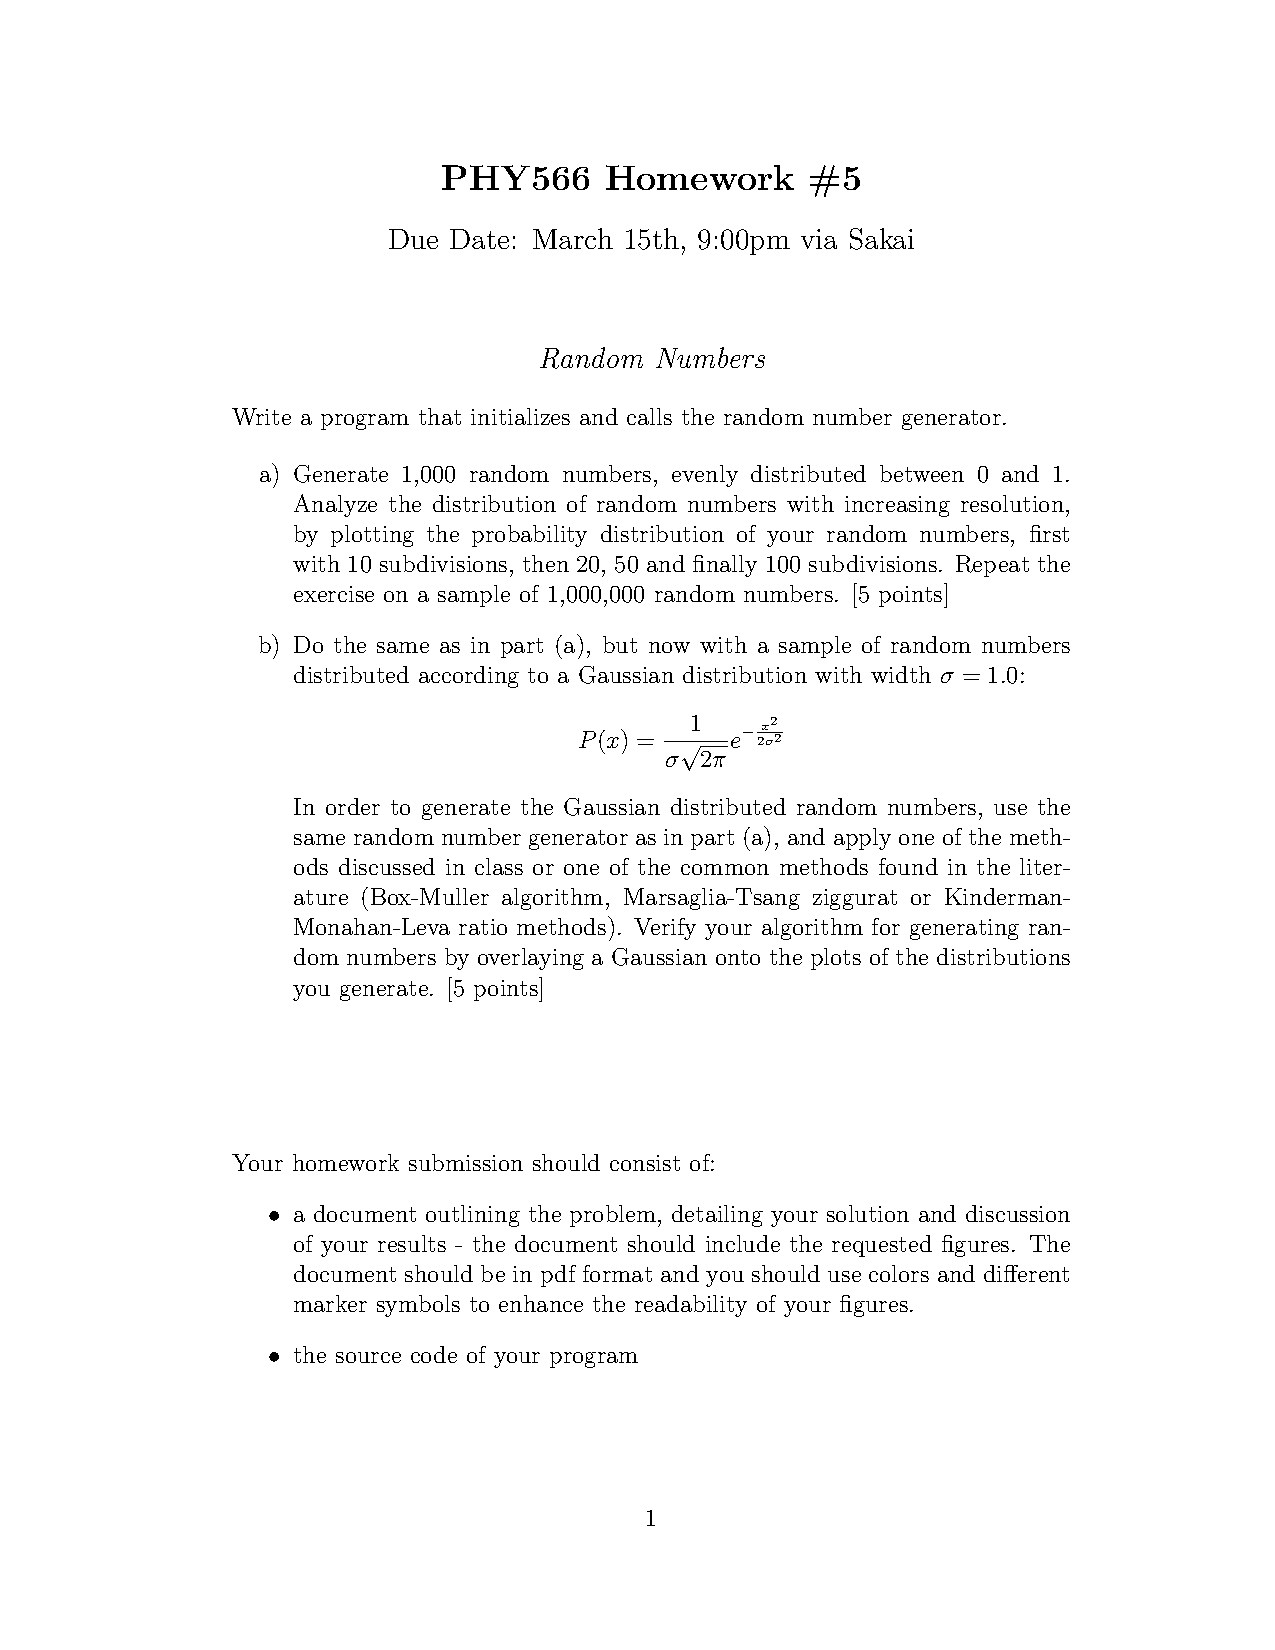
\includepdf{../homework5.pdf}

\clearpage
\section{Code}
\label{sec:code}

\lstinputlisting[style=python]{../code/random_numbers.py}

\end{document} %%% end of doc %%%
%%%%%%%%%%%%%%%%%%%%%%%%%%%%%%%%%%%%%%%%%%%%%%%%%%%%%


\bibliographystyle{bib_files/styles/atlasBibStyleWoTitle}
\bibliography{bib_files/my_bib.bib}

